\documentclass{beamer}

\usepackage[utf8]{inputenc}
\usepackage[T2A]{fontenc}
\usepackage[russian,english]{babel}
\usepackage{tikz}
\usetikzlibrary{positioning}
\usetikzlibrary{calc}
\usetikzlibrary{arrows}
\usetikzlibrary{decorations.pathmorphing,decorations.markings}
\usetikzlibrary{shapes}
\usetikzlibrary{patterns}
\usetikzlibrary{automata}
%\usetikzlibrary{tikzmark}
%\usetikzlibrary{calc}

\tikzset{
c/.style={
  circle,solid,
  inner sep=0pt,
  %text width=1mm,
  minimum width=7mm,
  align=center,
  draw=black,
  fill=white
  }
}


\newcommand{\tool}[1]{\texttt{#1}}
\newcommand*{\fx}{\ensuremath{\mathbf{x}}}%x}}}
\newcommand*{\fv}{\ensuremath{\mathbf{v}}} %v}}}
\newcommand{\defeq}{\ensuremath{=}}%\coloneqq}}%\Leftrightarrow}}%\triangleq}}

\usepackage{multicol}

\usepackage{fancyvrb}%fancy verbatim
%\makeatletter
%\newcommand{\verbatimfont}[1]{\renewcommand{\verbatim@font}{\ttfamily\scriptsize#1}}
%\makeatother
% redefine \VerbatimInput
\RecustomVerbatimCommand{\VerbatimInput}{VerbatimInput}{fontsize=\scriptsize}

\usepackage{pmboxdraw}
\usepackage{newunicodechar}
\newunicodechar{└}{\textSFii}
\newunicodechar{├}{\textSFviii}
\newunicodechar{─}{\textSFx}


\usepackage[export]{adjustbox} % loads also graphicx

\usepackage{listings}

\usepackage{subcaption}
\usepackage[font=scriptsize]{caption}
\setlength{\abovecaptionskip}{5pt plus 0pt minus 2pt} % Chosen fairly arbitrarily

\usepackage[backend=biber]{biblatex}
\addbibresource{../bib/ms-thesis.bib}
%\newcommand{\tikzmark}[1]{\tikz[remember picture] \node[coordinate] (#1) {#1};}

\usepackage{array}
\usepackage{xcolor}

\usepackage{hyphenat} % for using \nohyphens
%\usepackage{multirow} %Used for tables with merged cells
%\usepackage{collcell} %pdflatex.exe hangs without this one

\usepackage{booktabs}% http://ctan.org/pkg/booktabs
\newcommand{\tabitem}{~~\llap{\textbullet}~~}

\addtolength{\tabcolsep}{-3pt}
\setlength{\leftmargini}{10pt}
%\RequirePackage{aaltologo}
%\RequirePackage{beamercolorthemeAalto}
%\RequirePackage{beamerthemeAalto}

% There are many different themes available for Beamer. A comprehensive
% list with examples is given here:
% http://deic.uab.es/~iblanes/beamer_gallery/index_by_theme.html
% You can uncomment the themes below if you would like to use a different
% one:
%\usetheme[school={SCI}]{Aalto}
%\usetheme{AnnArbor}
%\usetheme{Antibes}
%\usetheme{Bergen}
%\usetheme{Berkeley}
%\usetheme{Berlin}
%\usetheme{Boadilla}
%\usetheme{boxes}
%\usetheme{CambridgeUS}
%\usetheme{Copenhagen}
%\usetheme{Darmstadt}
%\usetheme{default}
%\usetheme{Frankfurt}
%\usetheme{Goettingen}
%\usetheme{Hannover}
%\usetheme{Ilmenau}
%\usetheme{JuanLesPins}
%\usetheme{Luebeck}
%\usetheme{Madrid}
%\usetheme{Malmoe}
%\usetheme{Marburg}
%\usetheme{Montpellier}
%\usetheme{PaloAlto}
%\usetheme{Pittsburgh}
%\usetheme{Rochester}
\usetheme{Singapore}
%\usetheme{Szeged}
%\usetheme{Warsaw}

%\beamertemplatenavigationsymbolsempty  %no navigation bar
%\setbeamertemplate{footline}[frame number]
%\setbeamertemplate{headline}{}
\addtobeamertemplate{navigation symbols}{}{%
    \usebeamerfont{footline}%
    \usebeamercolor[fg]{footline}%
    \hspace{1em}%
    \insertframenumber/\inserttotalframenumber
}

\setbeamertemplate{frametitle}[default][left]
      
%\titlegraphic{\includegraphics[height=1cm,width=2cm]{logo1}}
%\titlegraphicii{\includegraphics[height=1cm,width=2cm]{logo2}}

\title{\nohyphens{\textbf{Automated~Analysis~of~Weak~Memory~Models}}}

% A subtitle is optional and this may be deleted
%\subtitle{Optional Subtitle}
\author{\textbf{Artem Yushkovskiy}\inst{1,2} \\ 
{\scriptsize MSc Candidate}
\\ \vspace{1em}
{\footnotesize\raggedleft Supervisors: \textbf{Assoc. Prof. Keijo Heljanko}\inst{1} \newline
\hphantom{Supervis} \textbf{Docent Igor I. Komarov}\inst{2} }
}%\small
%{\footnotesize%\raggedleft%does not work
%Supervisor 1: Assoc. Prof. Keijo Heljanko\inst{1} \newline
%Supervisor 2: Docent Igor I. Komarov\inst{2}
%}


\institute % (optional, but mostly needed)
{
  \inst{1}%
  Department of Computer Science, \\
  School of Science, \\
  \textbf{Aalto University} (Espoo, Finland)%
  \and
  \inst{2}%
  Faculty of Information Security \\
  and Computer Technologies, \\
  \textbf{ITMO University} (Saint Petersburg, Russia)%
}

\date{\scriptsize Espoo, Saint Petersburg, 2018}
% - Either use conference name or its abbreviation.
% - Not really informative to the audience, more for people (including
%   yourself) who are reading the slides online

%\subject{Computer Science}
% This is only inserted into the PDF information catalog. Can be left
% out. 

% If you have a file called "university-logo-filename.xxx", where xxx
% is a graphic format that can be processed by latex or pdflatex,
% resp., then you can add a logo as follows:

%\pgfdeclareimage[height=0.5cm]{university-logo}{}
%\logo{\pgfuseimage{university-logo}}

% Delete this, if you do not want the table of contents to pop up at
% the beginning of each subsection:
\AtBeginSection[]
{
  \begin{frame}<beamer>{Outline}
    \tableofcontents[currentsection]%,currentsubsection]
  \end{frame}
}

\usepackage{colortbl}

\definecolor{ltgrey}{rgb}{0.85,0.85,0.85}
\definecolor{dkblue}{rgb} {0,   0.1, 0.6}
\definecolor{dkred} {rgb} {0.6, 0.1, 0}
\renewcommand{\r}[1]{\ensuremath{\textcolor{dkred}{#1}}}
\renewcommand{\b}[1]{\ensuremath{\textcolor{dkblue}{#1}}}





% Let's get started
\begin{document}

\begin{frame}
  \titlepage
\end{frame}

\begin{frame}{Outline}
  \tableofcontents
\end{frame}




\section{Introduction}

\subsection{The problem}


\begin{frame}{Problem statement (Цель работы)}
To rework the proof-of-concept memory model-aware analysis tool \texttt{Porthos}~\cite{Porthos17a} by:
\begin{itemize}
\item extending the C-like input language,
\item revising its architecture and
\item re-implementing the tool in order to enhance performance, extensibility, reliability and maintainability
\end{itemize}
\end{frame}


\begin{frame}{Task specification (Задачи работы)}
\begin{itemize}
\item Study the general framework for memory model-aware analysis of concurrent programs~\cite{alglave2010shared};
\item Review existing tools for memory model-aware analysis;
\item Investigate existing architecture of \texttt{Porthos}, its strengths and weaknesses;
\item Design a new architecture for \texttt{PorthosC} that \textit{allow to} easily support the C input language, be robust, transparent, efficient and extensible.
\end{itemize}
\end{frame}


\subsection{The background: weak memory model-aware analysis}

\begin{frame}{Verification of concurrent software} {Example: Write-write reordering (compiler  relaxations)}
%1) mckenney  http://www.rdrop.com/users/paulmck/scalability/paper/whymb.2010.06.07c.pdf
%2) http://preshing.com/20120515/memory-reordering-caught-in-the-act/

\begin{table}
\centering
\ttfamily
\begin{tabular}{ |>{\color{dkblue}}c | >{\color{dkred}}c| }
\hline
\multicolumn{2}{|c|}{ \{ x=0; y=0; \}} \tabularnewline \hline
P & Q \\ \hline
$p_0$ : $x \leftarrow 1$   & $q_0$: $y \leftarrow 1$   \\
$p_1$ : $r_p \leftarrow y$ & $q_1$: $r_q \leftarrow x$ \\
\hline
\end{tabular}
\end{table}

%\tikzmark{p1} 
%\begin{tikzpicture}[remember picture, overlay]
%  \path[draw=red,thick,<->]<4-> (pic cs: p0) to [] (pic cs: p1);
%\end{tikzpicture}

\hspace{-20pt}
\begin{minipage}{.25\textwidth}
\small
\onslide<2-> 
\begin{table}
\caption*{SC}
\begin{tabular}{ >{\columncolor{ltgrey}}l >{\columncolor{ltgrey}}r}
$\b{p_0}, \b{p_1}, \r{q_0}, \r{q_1}$ & $(\b{0}; \r{1})$ \\
$\r{q_0}, \r{q_1}, \b{p_0}, \b{p_1}$ & $(\b{1}; \r{0})$
\onslide<3-> 
\\
$\b{p_0}, \r{q_0}, \b{p_1}, \r{q_1}$ & $(\b{1}; \r{1})$ \\
$\b{p_0}, \r{q_0}, \r{q_1}, \b{p_1}$ & $(\b{1}; \r{1})$ \\
$\r{q_0}, \b{p_0}, \b{p_1}, \r{q_1}$ & $(\b{1}; \r{1})$ \\
$\r{q_0}, \b{p_0}, \r{q_1}, \b{p_1}$ & $(\b{1}; \r{1})$ \\
\end{tabular}
\end{table}
\end{minipage}
\pause
%
\hspace{5pt}
\begin{minipage}{.6\textwidth}
\small
\onslide<4->
%\vspace{-1em}
%"delay the effect of a store past any load from a different location."
%\vspace{-11pt}
%\vspace{-2pt}
\begin{table}
\caption*{TSO}
\begin{tabular}{ | l r | l r | l r }
$\underline{\b{p_1}}, \underline{\b{p_0}}, \r{q_0}, \r{q_1}$ & $(\b{0}; \r{1})$  &  $\b{p_0}, \b{p_1}, \underline{\r{q_1}}, \underline{\r{q_0}}$ & $(\b{0}; \r{1})$  &  $\underline{\b{p_1}}, \underline{\b{p_0}}, \underline{\r{q_1}}, \underline{\r{q_0}}$ & $(\b{0}; \r{1})$ \\
$\r{q_0}, \r{q_1}, \underline{\b{p_1}}, \underline{\b{p_0}}$ & $(\b{1}; \r{0})$  &  $\underline{\r{q_1}}, \underline{\r{q_0}}, \b{p_0}, \b{p_1}$ & $(\b{1}; \r{0})$  &  $\underline{\r{q_1}}, \underline{\r{q_0}}, \underline{\b{p_1}}, \underline{\b{p_0}}$ & $(\b{1}; \r{0})$ \\
$\underline{\b{p_1}}, \r{q_0}, \underline{\b{p_0}}, \r{q_1}$ & $(\b{0}; \r{1})$  &  $\b{p_0}, \underline{\r{q_1}}, \b{p_1}, \underline{\r{q_0}}$ & $(\b{0}; \r{1})$  &  $\underline{\b{p_1}}, \underline{\r{q_1}}, \underline{\b{p_0}}, \underline{\r{q_0}}$ & $(\b{0}; \r{0})$ \\
$\underline{\b{p_1}}, \r{q_0}, \r{q_1}, \underline{\b{p_0}}$ & $(\b{0}; \r{0})$  &  $\b{p_0}, \underline{\r{q_1}}, \underline{\r{q_0}}, \b{p_1}$ & $(\b{1}; \r{1})$  &  $\underline{\b{p_1}}, \underline{\r{q_1}}, \underline{\r{q_0}}, \underline{\b{p_0}}$ & $(\b{0}; \r{0})$ \\
$\r{q_0}, \underline{\b{p_1}}, \underline{\b{p_0}}, \r{q_1}$ & $(\b{1}; \r{1})$  &  $\underline{\r{q_1}}, \b{p_0}, \b{p_1}, \underline{\r{q_0}}$ & $(\b{0}; \r{0})$  &  $\underline{\r{q_1}}, \underline{\b{p_1}}, \underline{\b{p_0}}, \underline{\r{q_0}}$ & $(\b{0}; \r{0})$ \\
$\r{q_0}, \underline{\b{p_1}}, \r{q_1}, \underline{\b{p_0}}$ & $(\b{1}; \r{0})$  &  $\underline{\r{q_1}}, \b{p_0}, \underline{\r{q_0}}, \b{p_1}$ & $(\b{1}; \r{0})$  &  $\underline{\r{q_1}}, \underline{\b{p_1}}, \underline{\r{q_0}}, \underline{\b{p_0}}$ & $(\b{0}; \r{0})$ \\
\end{tabular}
\end{table}
\end{minipage}

\end{frame}



\begin{frame}{Verification of concurrent software} {Example: Store buffering (hardware relaxations)}
\begin{center}
\scalebox{0.7}{
\ttfamily
\begin{tabular}{ |>{\color{dkblue}}c | >{\color{dkred}}c| }
\hline
\multicolumn{2}{|c|}{ \{ x=0; y=0; \}} \tabularnewline \hline
P & Q \\ \hline
$p_0$ : $x \leftarrow 1$   & $q_0$: $y \leftarrow 1$   \\
$p_1$ : $r_p \leftarrow y$ & $q_1$: $r_q \leftarrow x$ \\
\hline
\end{tabular}
}
\end{center}

\begin{figure}
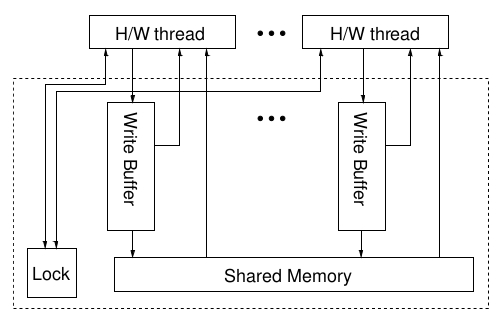
\includegraphics[scale=0.37]{img/x86-arch-full.png}
\caption{An x86-TSO abstract machine~\cite{sewell2010x86}}
%\label{fig:x86-arch}
\end{figure}
\end{frame}





\begin{frame}{The weak memory model} {Axiomatic semantics: The definition}

\begin{itemize}
  \addtolength{\tabcolsep}{0pt}
  \item \textbf{Event} $\in \mathbb{E}$, a low-level primitive operation:
    \begin{itemize}
      \item \textit{memory event} $\in \mathbb{M} = \mathbb{R} \cup \mathbb{W}$: access to a local/shared memory, \\
      \item \textit{computational event} $\in \mathbb{C}$: computation over local memory, and \\
      \item \textit{barrier event} $\in \mathbb{B}$: synchronisation fences;
     \end{itemize}
  \item \textbf{Relation} $\subseteq \mathbb{E} \times \mathbb{E}$: 
    \begin{itemize}
    \item \textit{basic relations}:%, computed from the program model:
      \begin{itemize}
        \item \textit{program-order} relation $\texttt{po} \subseteq \mathbb{E} \times \mathbb{E}$: (control-flow),
        \item \textit{read-from} relation $\texttt{rf} \subseteq \mathbb{W} \times \mathbb{R}$: (data-flow), and
        \item \textit{coherence-order} relation $\texttt{co} \subseteq \mathbb{W} \times \mathbb{W}$: (data-flow);
      \end{itemize}
    \item \textit{derived relations}:%, computed from the basic relations using the following operators:
      \begin{itemize}
        \item \textit{union} \texttt{r1\,|\,r2},
        \item \textit{sequence} \texttt{r1} ; \texttt{r2},
        %\item \textit{inverse} \texttt{r}\^{\texttt{-1}},
        \item \textit{transitive closure} \texttt{r+},
        \item $\cdots$;
      \end{itemize}
    \end{itemize}
  %\item \textbf{Candidate execution}, a sequence of guesses of relations;
  \item \textbf{Assertion} over relations or sets of events: 
    \begin{itemize}
    \item \textit{acyclicity}, \textit{irreflexivity} or \textit{emptiness} 
    \end{itemize}
\end{itemize}

\end{frame}



\begin{frame}{The weak memory model} {Testing the candidate executions}
\vspace{10pt}
\begin{minipage}{.3\linewidth}
\hfill
\end{minipage}
%
\noindent\begin{minipage}{.4\linewidth}
\scalebox{0.7}{
\ttfamily
\begin{tabular}{ |>{\color{dkblue}}c | >{\color{dkred}}c| }
\hline
\multicolumn{2}{|c|}{ \{ x=0; y=0; \}} \tabularnewline \hline
P & Q \\ \hline
$p_0$ : $x \leftarrow 1$   & $q_0$: $y \leftarrow 1$   \\
$p_1$ : $r_p \leftarrow y$ & $q_1$: $r_q \leftarrow x$ \\
\hline
\end{tabular}
}
\end{minipage}
%
\noindent\begin{minipage}{.25\linewidth}
\end{minipage}
\vspace{-5pt}
\begin{figure}
\centering
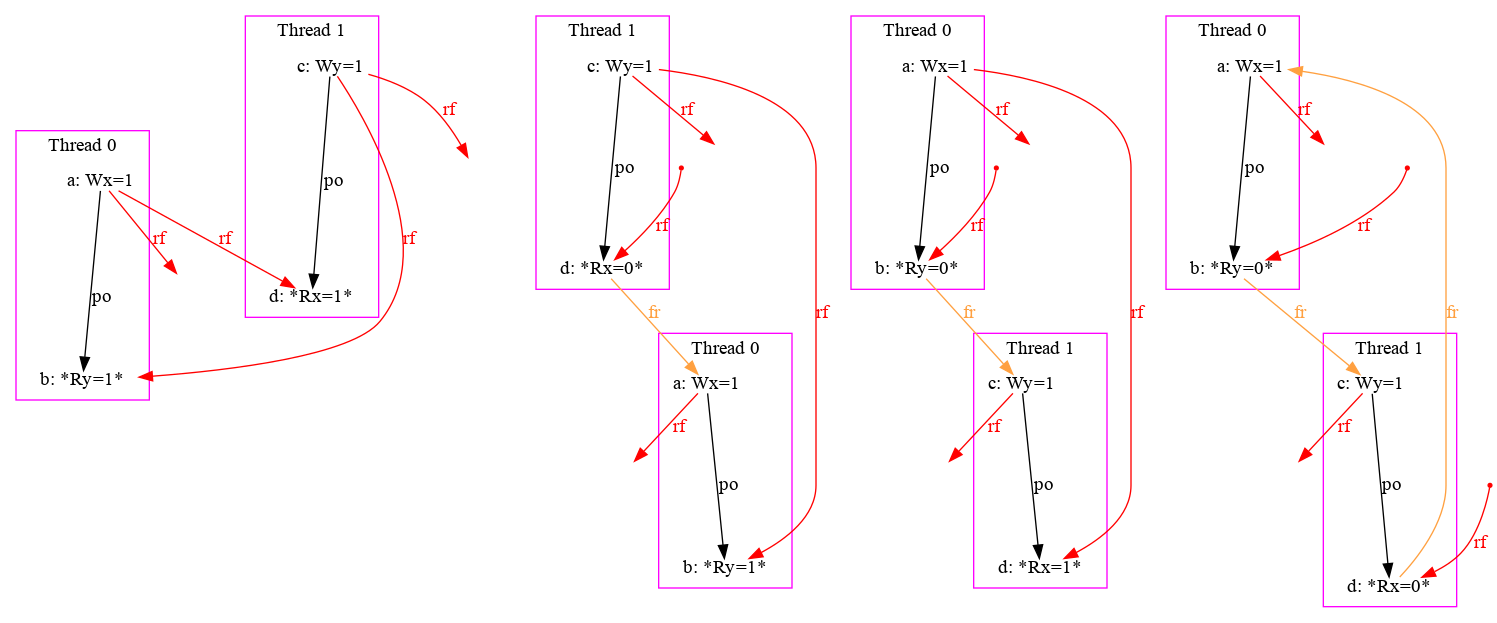
\includegraphics[width=\linewidth]{img/candidate.png}
\caption{The four candidate executions allowed under x86-TSO}
\end{figure}
\end{frame}




\begin{frame}{The weak memory model} {Testing the candidate executions}
\vspace{10pt}
\begin{minipage}{.3\linewidth}
\hfill
\end{minipage}
%
\noindent\begin{minipage}{.4\linewidth}
\scalebox{0.7}{
\ttfamily
\begin{tabular}{ |>{\color{dkblue}}c | >{\color{dkred}}c| }
\hline
\multicolumn{2}{|c|}{ \{ x=0; y=0; \}} \tabularnewline \hline
P & Q \\ \hline
$p_0$ : $x \leftarrow 1$   & $q_0$: $y \leftarrow 1$   \\
$p_1$ : $r_p \leftarrow y$ & $q_1$: $r_q \leftarrow x$ \\
\hline
\end{tabular}
}
\end{minipage}
%
\raggedleft{
\noindent\begin{minipage}{.25\linewidth}
\scriptsize
SC model: \\
... \\
\texttt{fr = (rf\^\,-1; co)} \\
\color{red}\texttt{acyclic(fr $\cup$ po)}
\end{minipage}
}
\vspace{-5pt}
\begin{figure}
\centering
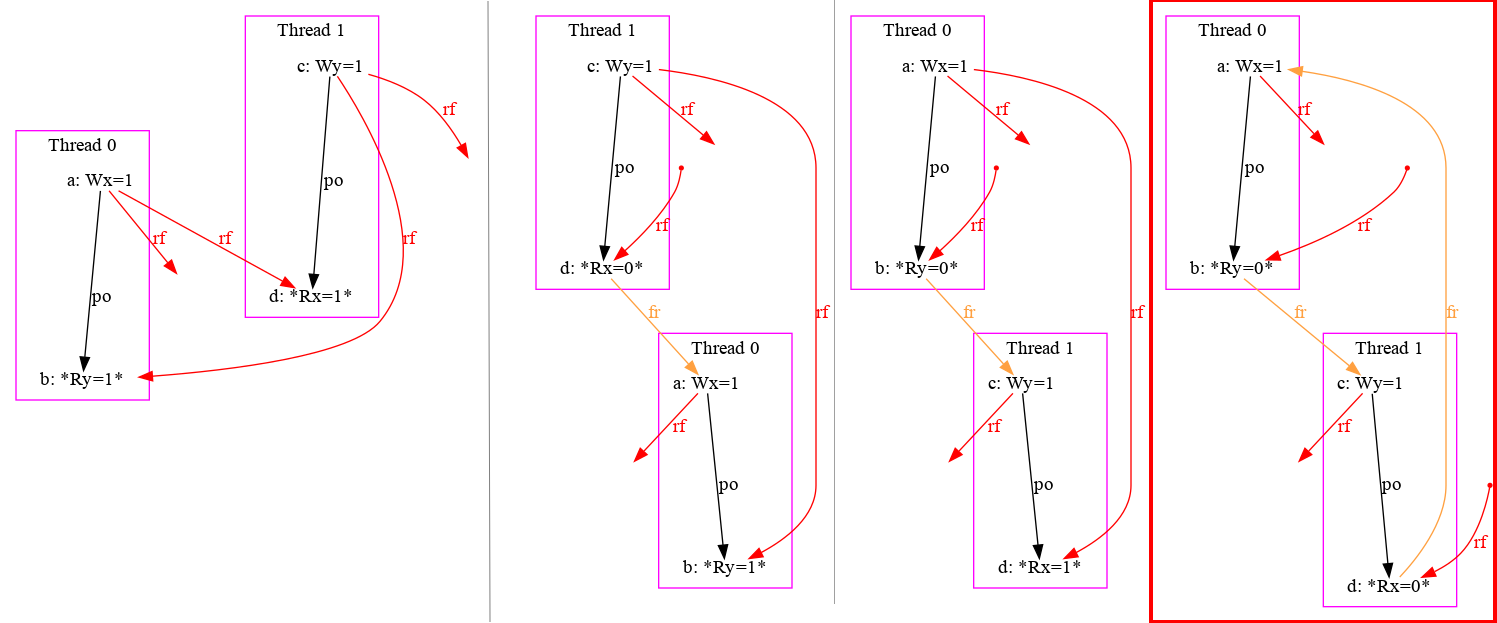
\includegraphics[width=\linewidth]{img/candidate-red.png}
\caption{The four candidate executions allowed under x86-TSO}
\end{figure}

\end{frame}











\begin{frame}{Tools for memory model-aware analysis}
\begin{itemize}
\item \texttt{diy} tool suite:
  \begin{itemize}
  \item \tool{diy}, \tool{diycross} and \tool{diyone}, litmus tests generators,
  \item \tool{litmus}, a litmus test concrete executor, and 
  \item \tool{herd}, a weak memory model simulator;
  \end{itemize}
%\item the stateless model checkers (\tool{CHESS}~\cite{musuvathi2008fair}, \tool{Nidhugg}~\cite{abdulla2017stateless}); %TODO: description of statelessses
\item the stateless model checkers (\tool{CHESS}, \tool{Nidhugg}); %TODO: description of statelessses
\item the tool for automated synthesis of the synchronisation primitives \tool{musketeer};
\item the instrumenting compiler \tool{goto-cc} which is a part of \tool{CBMC} model checker;
\item the tool \texttt{Porthos} for analysing the portability of the C programs;
\item and others.
\end{itemize}
\end{frame}


\subsection{Portability Analysis}

\begin{frame}{Portability analysis} {The \texttt{Porthos} tool}

\begin{itemize}
\item Let the function $\textit{cons}_{\mathcal{M}}(P)$ calculate the set of executions of program $P$ consistent under the memory model $\mathcal{M}$.
\end{itemize}

\begin{definition}[Portability~\cite{Porthos17a}]
Let $\mathcal{M_S}$, $\mathcal{M_T}$ be two weak memory models.
The program $P$ is portable from $\mathcal{M_S}$ to $\mathcal{M_T}$ if 
$\textit{cons}_{\mathcal{M_T}}(P) \subseteq \textit{cons}_{\mathcal{M_S}}(P)$
\end{definition}

\begin{itemize}
\item Portability as an SMT-based bounded reachability problem: \\
${\phi = \phi_{CF} \land \phi_{DF} \land \phi_{\mathcal{M_T}} \land \phi_{\lnot\mathcal{M_S}}}$
\item $\texttt{SAT}(\phi) \implies $ the portability bug
\end{itemize}

%end{tabular}
\end{frame}



\subsection{SMT-encoding}


%\begin{frame}{Encoding for the control-flow}% {The \texttt{Porthos v1} encoding scheme}
%\begin{itemize}
%\item In \texttt{Porthos}, the high-level instructions were represented in the SMT-formula by separate variables.
%\item For example, the sequential instruction $i_1 = i_2; i_3$ was encoded as
%$\phi_{CF}(i_2;i_3) = (cf_{i_1} \Leftrightarrow (cf_{i_2} \land cf_{i_3})) \land \phi_{CF}(i_2) \land \phi_{CF}(i_3)$,
%\end{itemize}
%\end{frame}

%\begin{frame}{Encoding for the control-flow}% {The \texttt{PorthosC} encoding scheme}
%\begin{itemize}
%%\item The new encoding scheme of \texttt{PorthosC} follows~\cite{heljanko2008unfoldings} in general.
%\item \texttt{Porthos v1} used another encoding scheme, where the high-level instructions were represented in the SMT-formula by separate variables:
%$\phi_{CF}(i_2;i_3) = (cf_{i_1} \Leftrightarrow (cf_{i_2} \land cf_{i_3})) \land \phi_{CF}(i_2) \land \phi_{CF}(i_3)$.
%\item In \texttt{PorthosC}, the high-level AST firstly is compiled into the \textit{event-flow graph} with events as nodes and relations as edges.
%\item All edges are labelled by \textit{guards}, local-memory computations ($\epsilon$~denotes an empty guard).
%\end{itemize}
%
%\begin{figure}[b]
%  \centering
%  \begin{minipage}{\textwidth}
%      \begin{subfigure}[b]{0.25\textwidth}
%        \makebox[\textwidth]{
%        \begin{tikzpicture}[->,>=stealth',shorten >=1pt,auto,node distance=1.5cm,semithick]
%            \node[c] (1) [] {$e_i$};
%            \node[c] (2) [below of=1] {$e_{i+1}$};
%            \path[->]
%            (1) edge [] node {$\epsilon$} (2)
%            ;
%        \end{tikzpicture}
%        }
%        \caption{The sequence}
%    \end{subfigure}
%    ~
%    \begin{subfigure}[b]{0.35\textwidth}
%        \makebox[\textwidth] {
%        \begin{tikzpicture}[->,>=stealth',shorten >=1pt,auto,node distance=1.5cm,semithick]
%            \node[c]           (k)   [] {$e_k$};
%            \node[c,draw=none] (iii) [below of=k] {$...$};
%            \node[c,draw=none] (ii)  [left=0.2cm of iii] {};
%            \node[c]           (i)   [left=0.2cm of ii] {$e_i$};
%            \node[c,draw=none] (iv)  [right=0.2cm of iii] {};
%            \node[c]           (v)   [right=0.2cm of iv] {$e_{i+j}$};
%            \path[->]
%            (k) edge [above] node {$g_{i,k}$} (i)
%            (k) edge [] node {} (ii)
%            (k) edge [] node {} (iii)
%            (k) edge [] node {} (iv)
%            (k) edge [above] node {$g_{i+j,k}$} (v)
%            ;
%        \end{tikzpicture}
%        }
%        \caption{Conditional branching}
%    \end{subfigure}
%    ~
%    \begin{subfigure}[b]{0.3\textwidth}
%        \makebox[\textwidth]{
%        \begin{tikzpicture}[->,>=stealth',shorten >=1pt,auto,node distance=1.5cm,semithick]
%            \node[c] (i) [] {$e_i$};
%            \node[c,draw=none] (ii) [right=0.2cm of i] {};
%            \node[c,draw=none] (iii) [right=0.2cm of ii] {$...$};
%            \node[c,draw=none] (iv) [right=0.2cm of iii] {};
%            \node[c] (v) [right=0.2cm of iv] {$e_{i+j}$};
%            \node[c] (k) [below of=iii] {$e_k$};
%            \path[->]
%            (i) edge [above] node {$g_{i,k}$} (k)
%            (ii) edge [above] node {} (k)
%            (iii) edge [] node {} (k)
%            (iv) edge [] node {} (k)
%            (v) edge [] node {} (k) %sloped
%            ;
%        \end{tikzpicture}
%        }
%        \caption{Branch merging}
%    \end{subfigure}
%    %
%    \caption{Possible mutual arrangements of events in a control-flow graph} %Linear and non-linear cases of a control-flow graph}
%    \label{encode:cf}
%\end{minipage}
%\end{figure}
%\end{frame}


%\begin{frame}{Encoding for the control-flow} %{The \texttt{PorthosC} encoding scheme}
%\begin{itemize}
%\item Let $\fx:\,\mathbb{E}\,\rightarrow\,\{0,1\}$ be the predicate that signifies the fact that the event has been e\textbf{x}ecuted.
%\item The control-flow of the program is encoded as following:
%\end{itemize}
%\vspace{-20pt}
%\begin{align}
%\phi_{CF_{seq}} \defeq \quad & \fx(e_{i+1}) \Rightarrow \fx(e_i) \nonumber\\
%\phi_{CF_{br}}  \defeq \quad & [\fx(e_i) \Rightarrow \fx(e_k)] \ \land \ \cdots \ \land \ [\fx(e_{i+j}) \Rightarrow \fx(e_k)] \nonumber \nonumber\\
%                       \land & \ [\fx(e_i) \land \fx(e_k) \Rightarrow g_{i,k}] \ \land \ \cdots \ \land \ [\fx(e_{i+j}) \land \fx(e_k) \Rightarrow g_{i+j,k}] \nonumber \\
%                       \land & \ \cdots \nonumber \nonumber\\
%                       \land & \ ( \bigvee_{e_l \in \ \texttt{succ}(e_m)} \ \ \bigvee_{\begin{subarray}{l}e_n \in \ \texttt{succ}(e_k) \nonumber\\
%                               e_n \neq e_m\end{subarray}} \! \lnot [\fx(e_m) \land \fx(e_n)] \ ) \nonumber\\
%\phi_{CF_{mer}} \defeq \quad & \fx(e_k) \Rightarrow (\bigvee\limits_{e_p \in \ \texttt{pred}(e_k)}^{} \fx(e_p)) \nonumber
%\end{align}
%\end{frame}



\begin{frame}{Encoding for the control-flow: An example}
%Let $\fx:\,\mathbb{E}\,\rightarrow\,\{0,1\}$ be the predicate that signifies the fact that the event has been e\textbf{x}ecuted (and, consequently, has changed the state of the system).
\begin{figure}
\begin{minipage}{.2\textwidth}
\centering
\begin{tikzpicture}[->,>=stealth',shorten >=1pt,auto,node distance=1.5cm,semithick]
    \node[c] (i)   [] {$e_1$};
    \node[c] (ii)  [below of=i] {$e_2$};
    \node[c,fill=black!15] (lnop) [below left = 0.25cm and 0.7cm of ii] {$e_{nop_{1}}$};
    \node[c] (iii) [below of=ii] {$e_3$};
    \node[c,fill=black!15] (rnop) [right = 0.4cm of iii] {$e_{nop_{2}}$};
    \node[c] (iv)  [below of=iii] {$e_4$};
    \path[->]
    (i) edge [right] node {$\epsilon$} (ii)
    (i) edge [right,bend right=25] node {$g_{1,4}$} (lnop)
    (lnop) edge [right,bend right=25] node {$\epsilon$} (iv)
    (ii) edge [right] node {$g_{2,3}$} (iii)
    (iii) edge [right] node {$\epsilon$} (iv)
    (ii) edge [right,bend left=25] node {$g_{2,4}$} (rnop)
    (rnop) edge [right,bend left=25] node {$\epsilon$} (iv)
    ;
\end{tikzpicture}
\end{minipage}
%
\hspace{15pt}
\begin{minipage}{.4\textwidth}
\centering
\begin{align*}
\phi_{CF} \defeq \ & [\fx(e_2) \Rightarrow \fx(e_1)] \\
                 \ & \land [\fx(e_3) \Rightarrow \fx(e_2)] \\
                 \ & \land [\fx(e_{nop_{1}}) \Rightarrow \fx(e_1)] \\
                 \ & \land [\fx(e_{nop_{2}}) \Rightarrow \fx(e_2)] \\
                 \ & \land [\fx(e_4) \Rightarrow (\fx(e_{nop_{1}}) \lor \fx(e_3) \lor \fx(e_{nop_{2}}))] \\
                 \ & \land [\fx(e_{nop_{1}}) \land \fx(e_1) \Rightarrow g_{1,4}] \\
                 \ & \land [(\fx(e_3) \land \fx(e_2)) \Rightarrow g_{2,3}] \\
                 \ & \land [(\fx(e_{nop_{2}}) \land \fx(e_2)) \Rightarrow g_{2,4}] \\
                 \ & \land \lnot [\fx(e_2) \land \fx(e_{nop_{1}})] \\
                 \ & \land \lnot [\fx(e_3) \land \fx(e_{nop_{2}})]
\end{align*}
\end{minipage}
\caption{Example of encoding for the control-flow of the event-flow graph}
\end{figure}
\end{frame}



\begin{frame}{Encoding for the data-flow}
\begin{itemize}
\item SSA-indices are computed as following:
\begin{itemize}
  \item any access to a shared variable (both read and write) increments its SSA-index;
  \item only writes to a local variable increment its SSA-index (reads preserve indices);
  \item no access to a constant variable or computed (evaluated) expression changes their SSA-index.
\end{itemize}
\end{itemize}
The data-flow of an event is encoded as following:
\begin{align}
    \phi_{DF_{e = \texttt{load}(r \leftarrow l)}}  \defeq \ & [\fx(e) \Rightarrow (r_{i+1} = l_{i+1})] \nonumber \\
    \phi_{DF_{e = \texttt{store}(l \leftarrow r)}} \defeq \ & [\fx(e) \Rightarrow (l_{i+1} = r_i)] \nonumber\\
    \phi_{DF_{e = \texttt{eval}(\cdot)}}           \defeq \ & [\fx(e) \Rightarrow \fv(e)] \nonumber \\
\end{align}
%    \phi_{DF_{mem}}(e_1, e_2) \defeq \ & [\texttt{rf}(e_1, e_2) \Rightarrow (l_i = l_j)] \nonumber
\end{frame}




\section{Implementation}

%\begin{frame}{General principles}
%\begin{enumerate}[nolistsep]
%  \item \textit{Robustness:}
%    \begin{enumerate}[label*=\arabic*.]
%      \item preservation the completeness of analysis,
%      \item modular architecture: each module can be tested independently,
%      \item usage of software design patterns where necessary, and
%      \item usage of immutable data structures for all DTOs.
%    \end{enumerate}
%  \item \textit{Transparency:}
%    \begin{enumerate}[label*=\arabic*.]
%      \item following the principles of simplicity and readability, and
%      \item clear and informative program output.
%    \end{enumerate}
%  \item \textit{Efficiency:}
%    \begin{enumerate}[label*=\arabic*.]%[leftmargin=1.5em]
%      \item keeping the trade-off between execution time and memory usage.
%    \end{enumerate}
%  \item \textit{Extensibility:}
%    \begin{enumerate}[label*=\arabic*.]%[leftmargin=1em]
%      \item clear modular architecture.
%    \end{enumerate}
%\end{enumerate}
%\end{frame}


\subsection{The input language and general architecture}


\begin{frame}{The input language}
The input language parser used by \texttt{Porthos} suffered from several disadvantages:
\begin{itemize}
\item it contained the parser code inlined directly into the grammar (hardly maintainable);
\item the semantics of operations and kinds of variables (global or shared) were determined syntactically (4 different types of assignment:`\texttt{=}', `\texttt{:=}', `\texttt{<-}' and `\texttt{<:-}', each for different kinds of arguments);
\item restricted syntax for expressions.
\item In contrast, \texttt{PorthosC} uses the full C language grammar of proposed in the C11 standard~\cite{jtc2011sc22} and the visitor that converts the ANTLR grammar to the AST (\texttt{Y-tree}).
\end{itemize}

\end{frame}


\begin{frame}{Architecture}%{The general architecture}
\vspace{-30pt}
\begin{figure}
  \centering
  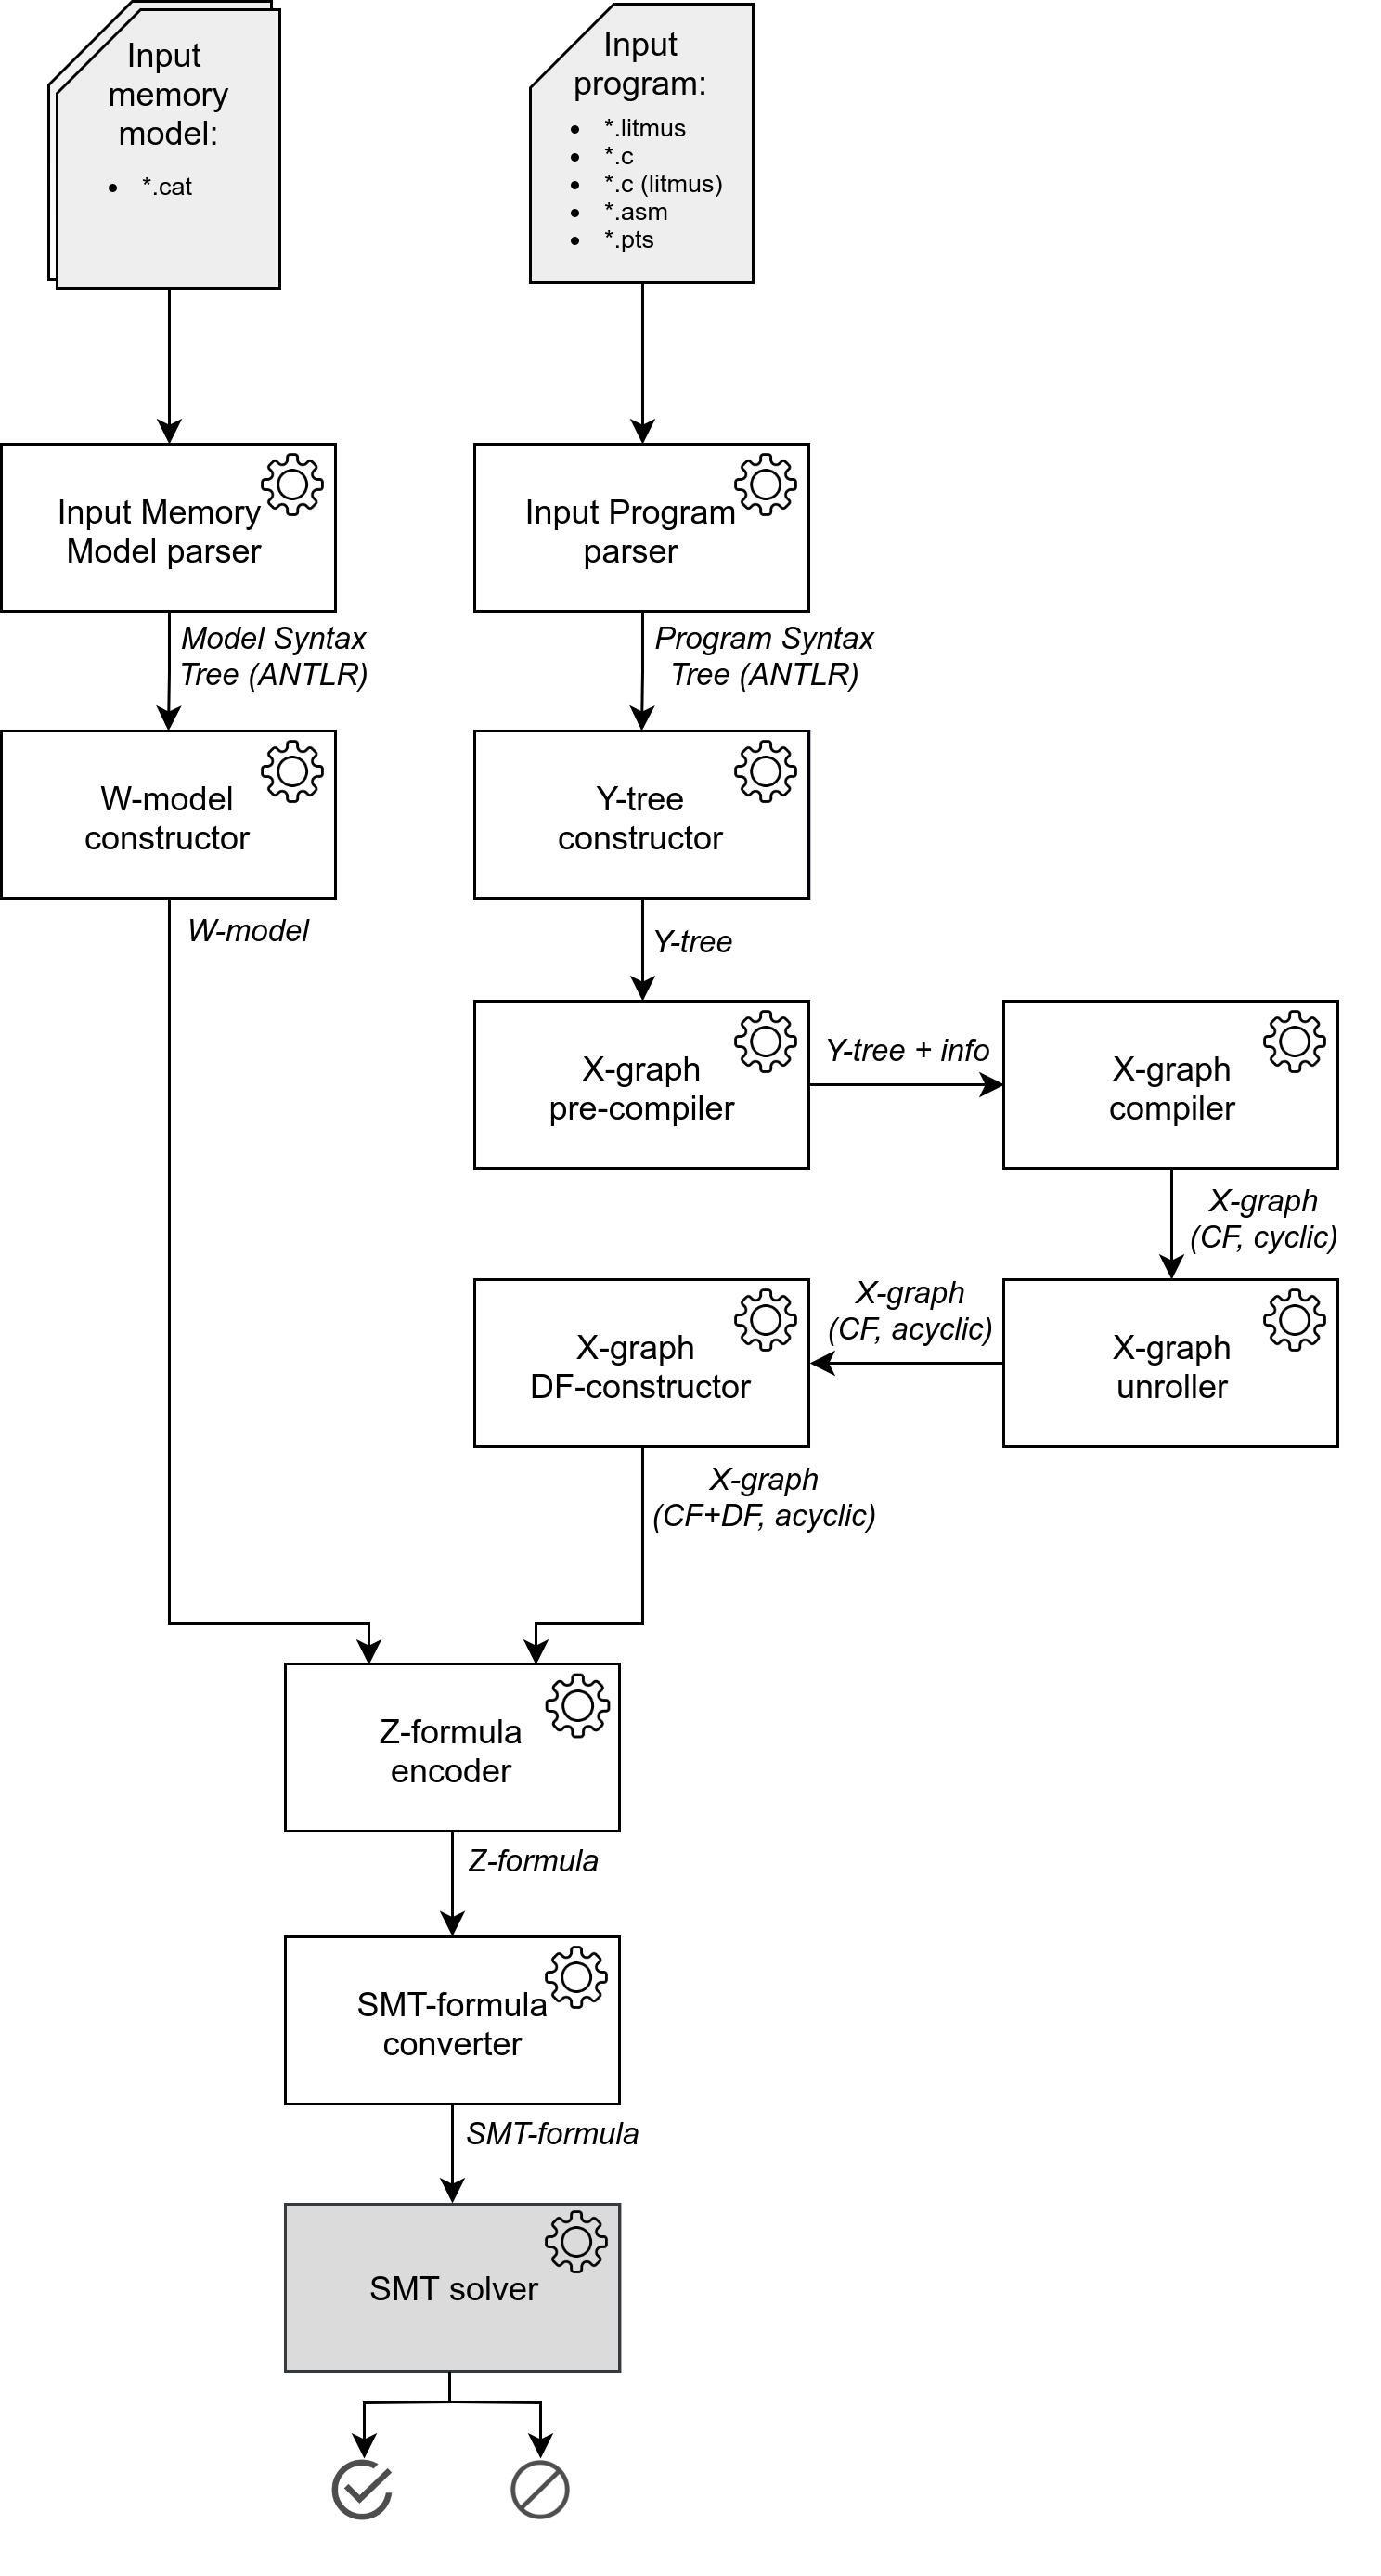
\includegraphics[height=.99\textheight,keepaspectratio]{../img/my/draw.io/general_arch-no_numbering.png} %{img/my/draw.io/general_arch.png}
  %\caption{The general architecture of \texttt{PorthosC}}
  %\label{fig:arch}
\end{figure}
\end{frame}




\subsection{The \texttt{X-graph}: structure and construction}

\begin{frame}{The \texttt{X-graph} internal representation}
  \centering
  \begin{figure}
    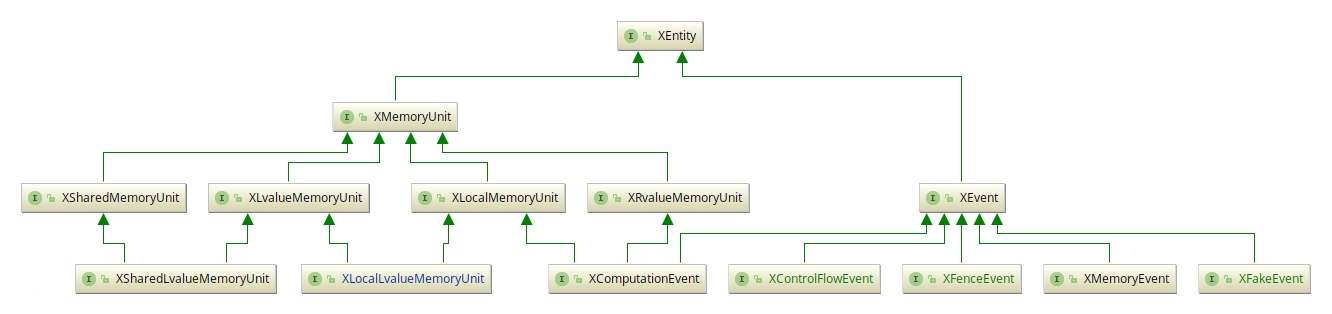
\includegraphics[width=1.1\textwidth,keepaspectratio]{../img/my/class-diagrams/XEntity-interfaces.png}
    \caption{The inheritance tree of main \texttt{X-graph} interfaces}
  \end{figure}
  
\end{frame}


\begin{frame}{The \texttt{X-graph} compiler}
\begin{figure}
  \centering
  \scalebox{0.7}{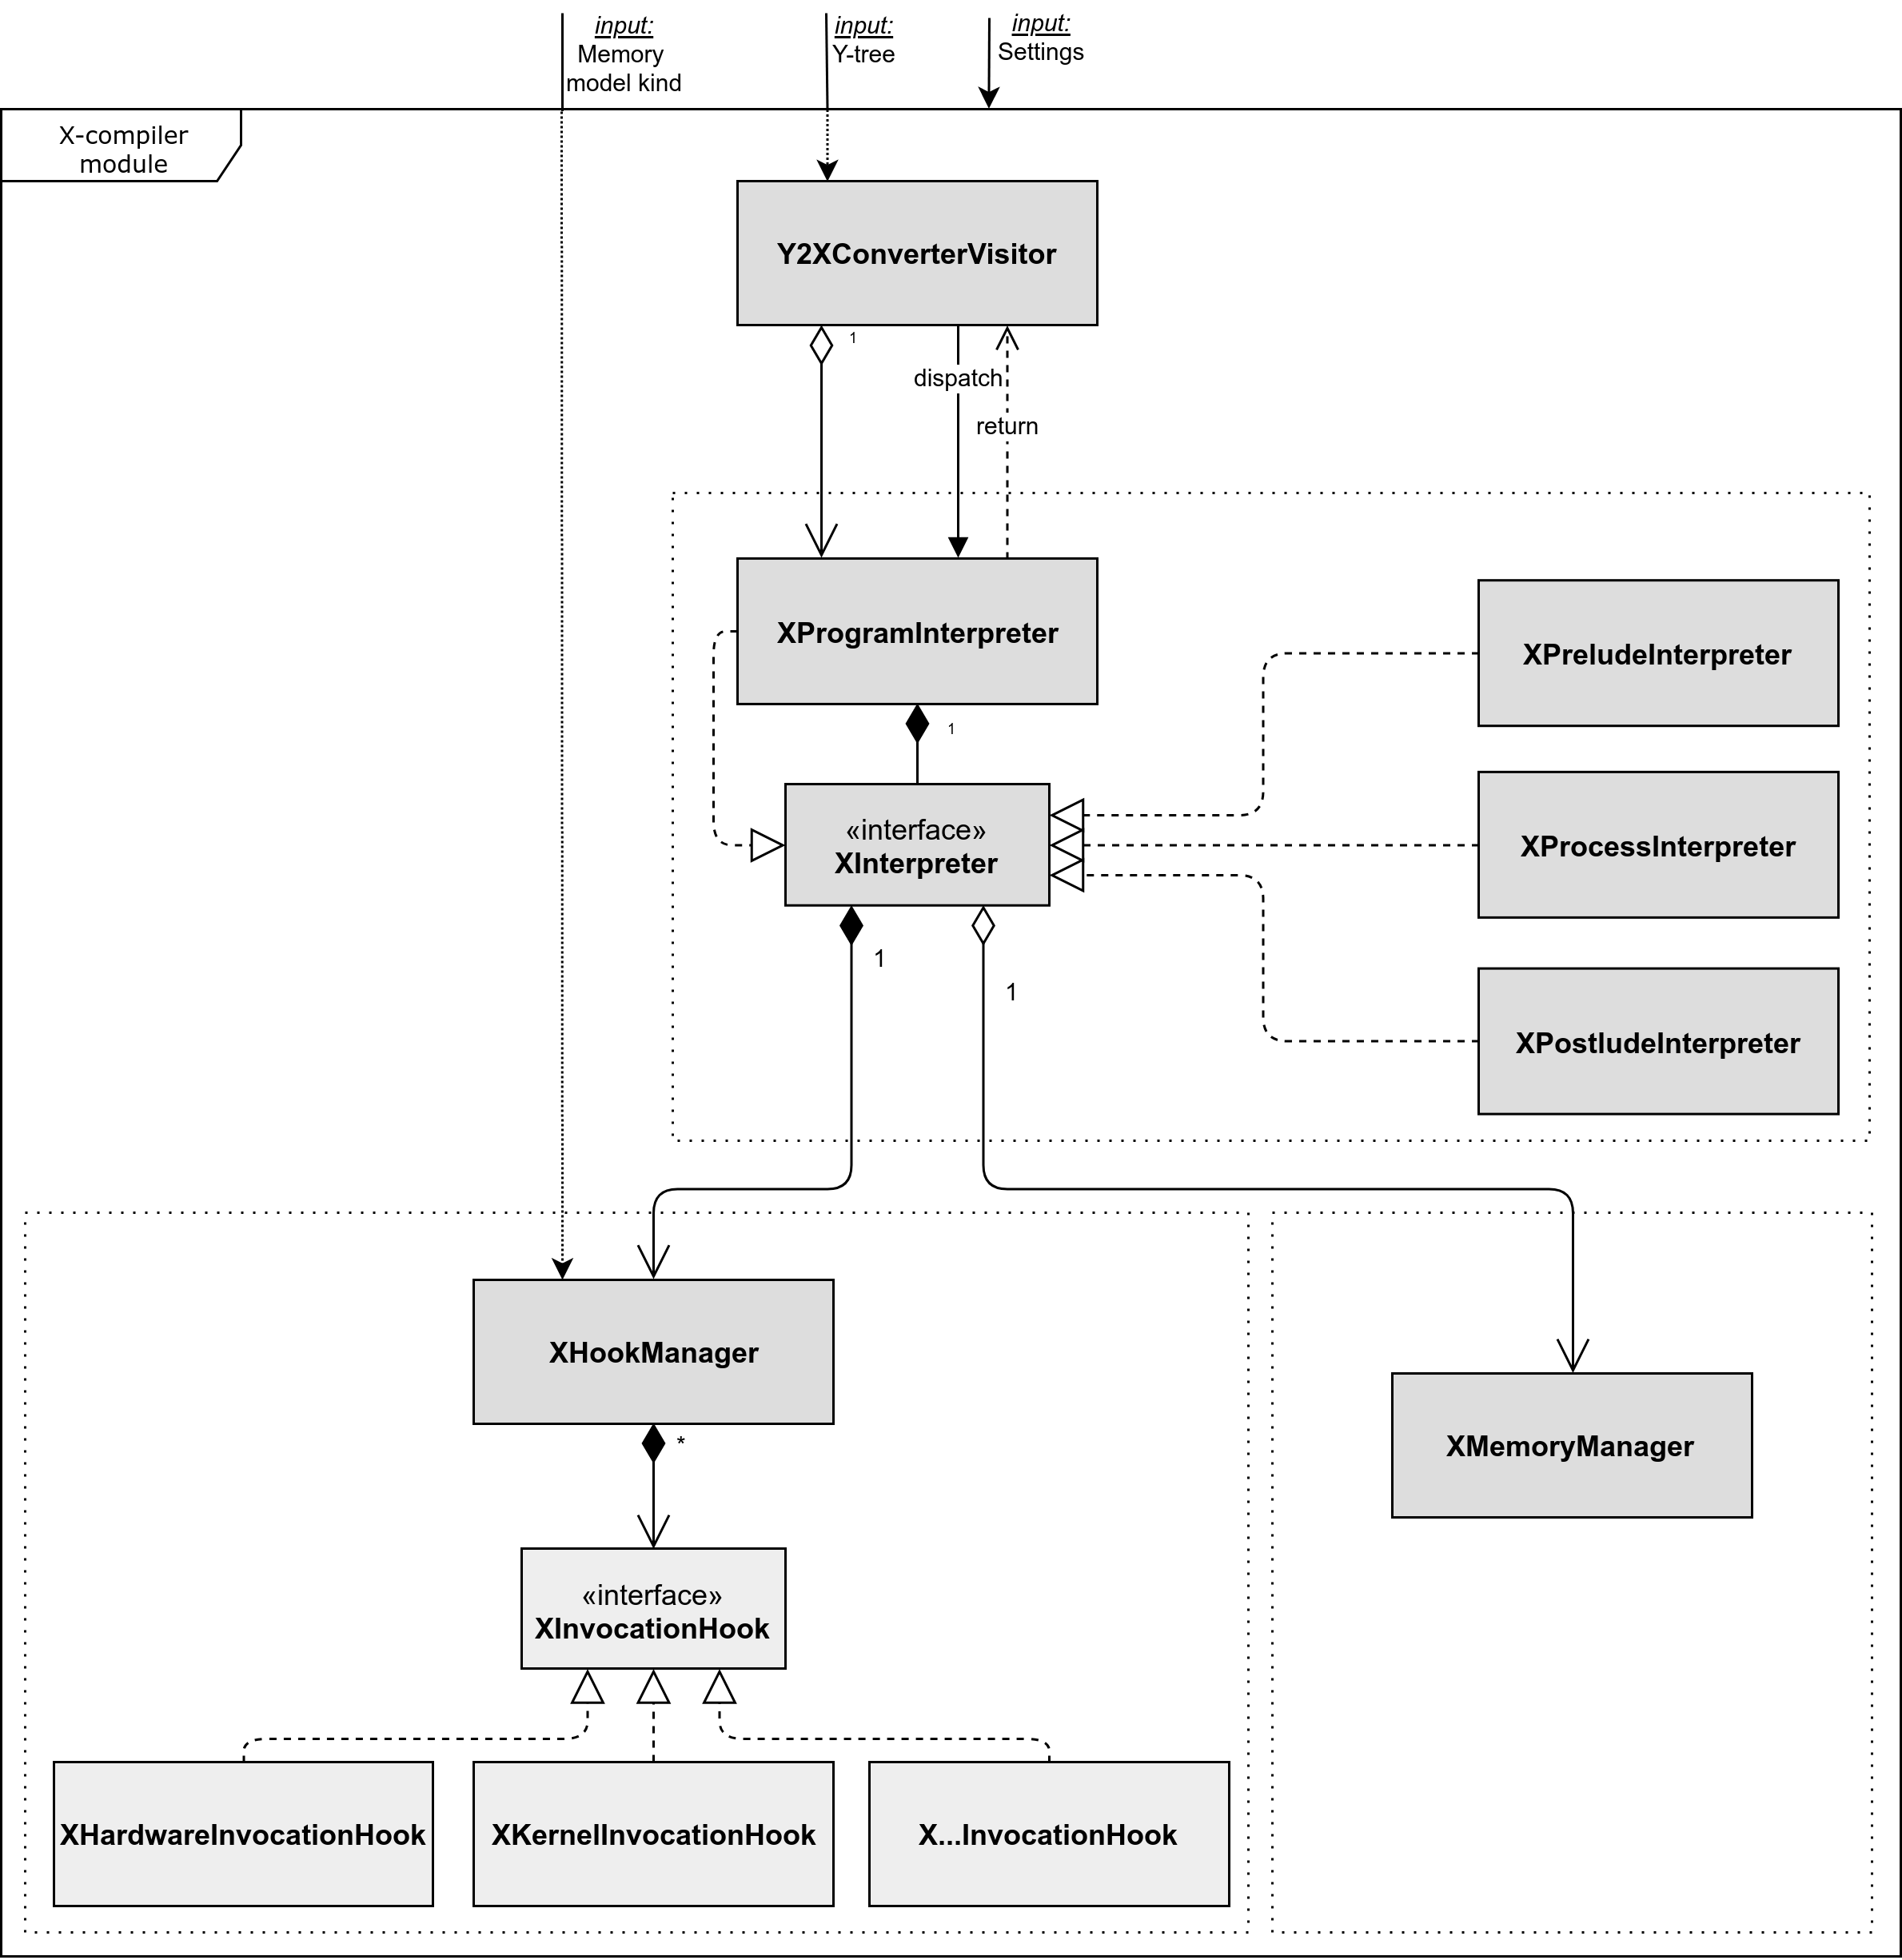
\includegraphics[height=.99\paperheight]{../img/my/draw.io/X-compiler.png}}
  \caption{Main components of the X-compilation processing unit}
\end{figure}
\end{frame}



\begin{frame}{\texttt{X-graph} unrolling}
\begin{figure}[t]
\centering
\resizebox{.8\linewidth}{!}{
\begin{tikzpicture}[->,>=stealth',shorten >=1pt,auto,node distance=1.5cm,semithick]
\node[c] (1) [] {$1$};
\node[c] (2) [below left of=1] {$2$};
\node[c] (3) [below right of=1] {$3$};
\node[c] (4) [below of=3] {$4$};
\path[->]
(1) edge [] node {} (2)
(2) edge [bend left=50,dotted] node {} (1)
(1) edge [] node {} (3)
(3) edge [] node {} (4)
(4) edge [bend right=80,dotted] node {} (1)
;
\node[draw=none] (impl) [right=3cm of 3] {$\overset{k = 6}{\longmapsto}$};
;
\node[c] (22) [right=3cm of impl] {$2_2$};
\node[c] (11) [above right=1cm and 1cm of 22]{$1_1$};
\node[c] (32) [below right=1cm and 1cm of 11] {$3_2$};
\node[c] (43) [below of=32] {$4_3$};
\node[c] (13) [below of=22] {$1_3$};
\node[c] (24) [below left=1cm and 1cm of 13] {$2_4$};
\node[c] (34) [below right=1cm and 1cm of 13] {$3_4$};
\node[c] (14) [below of=43] {$1_4$};
\node[c] (15) [below of=24] {$1_5$};
\node[c] (45) [below of=34] {$4_5$};
\node[c] (25) [below of=14] {$2_5$};
\node[c] (35) [below of=14] {$3_5$};
\node[c] (26) [below left=1cm and 1cm of 15] {$2_6$};
\node[c] (36) [below right=1cm and 1cm of 15] {$3_6$};
\node[c] (16) [below right=1cm and 0.2cm of 45] {$1_6$};
\node[c] (46) [below right=1cm and 0.3cm of 35] {$4_6$};
\node[rectangle,draw] (6) [below left=1cm and 1cm of 16] {$S$};
\node[] (k1) [right=3.2cm of 11] {$(k = 1)$};
\node[] (k2) [right=1.7cm of 32] {$(k = 2)$};
\node[] (k3) [right=1.7cm of 43] {$(k = 3)$};
\node[] (k4) [right=1.7cm of 14] {$(k = 4)$};
\node[] (k5) [right=1.7cm of 35] {$(k = 5)$};
\node[] (k6) [right=1cm of 46] {$(k = 6)$};
\path[->]
(11) edge [] node {} (22)
(11) edge [] node {} (32)
(32) edge [] node {} (43)
(22) edge [] node {} (13)
(13) edge [bend right=10] node {} (24)
(13) edge [bend left=10] node {} (34)
(43) edge [] node {} (14)
(24) edge [] node {} (15)
(34) edge [] node {} (45)
(14) edge [] node {} (25)
(14) edge [] node {} (35)
(15) edge [bend right=10] node {} (26)
(15) edge [bend left=10] node {} (36)
(45) edge [] node {} (16)
(35) edge [bend right=10] node {} (16)
(35) edge [bend left=10] node {} (46)
(26) edge [bend right=10] node {} (6)
(36) edge [bend right=5] node {} (6)
(16) edge [bend left=20] node {} (6)
(46) edge [bend left=20] node {} (6)
;
\end{tikzpicture}
}
\caption{Example of the flow graph unrolling up to bound $k = 6$}
\end{figure}
\end{frame}



\section{Evaluation}

\begin{frame}{Evaluation}
\alert{[to be done]}
\end{frame}




\section*{Summary}

\begin{frame}{Summary}
\begin{itemize}
\item The general framework for memory model-aware analysis was implemented in \texttt{PorthosC};
%\item Review existing tools for memory model-aware analysis;
\item The input language has been extended; %TODO: how exactly?
\item The old architecture of \texttt{Porthos} has been analysed and considered while designing the new architecture for \texttt{PorthosC};
%\item Design a new architecture for \texttt{PorthosC} that \textit{allow to} easily support the C input language, be robust, transparent, efficient and extensible.
\item \alert{to be done: more}
%\item the new architecture for the tool was designed,
\end{itemize}
\end{frame}



% All of the following is optional and typically not needed. 
\appendix
\section<presentation>*{\appendixname}
\subsection<presentation>*{For Further Reading}

\begin{frame}[allowframebreaks]
  \frametitle<presentation>{Bibliography}
  \printbibliography
\end{frame}

\end{document}


